\documentclass[12pt,a4paper]{article}
\usepackage[utf8]{inputenc} 
\usepackage[T1]{fontenc}		       
\usepackage{lmodern}			       
\usepackage{babel} 
\usepackage{amsmath}
\usepackage{amsfonts}
\usepackage{amssymb}
\usepackage{graphicx}
\usepackage{xcolor}
\usepackage{mathtools}
\usepackage{fancyhdr}
\usepackage{enumitem}
\usepackage{tcolorbox}
\usepackage{stmaryrd}
\usepackage{dsfont}
\usepackage{pgf, tikz}
\usetikzlibrary{shapes.misc}
\usepackage[linesnumbered,ruled,vlined]{algorithm2e}
\usepackage[text={15cm,24.5cm},centering]{geometry}


% Définir le texte affiché en fin de page
\pagestyle{fancy}
\fancyhf{}  % Clear the default headers and footers
\rfoot{\hrule
    \vspace{0.3cm}
    \noindent\textsf{Félix de Brandois}
    \hfill \thepage
}
\renewcommand{\headrulewidth}{0pt}

% Style de l'entete
\newcommand{\entete}{
    \noindent\textbf{INSA - ModIA, 5$^e$ année.}
    \hfill \textbf{Années 2024-2025}
    
    \begin{center}
        \textbf{\LARGE Analyse Mathématique et principes de la méthode}
    \end{center}
}


% Définir la fonction pour créer une boîte de propriété
\newcommand{\propriete}[2]{%
    \begin{tcolorbox}[colback=white,colframe=green!25!white,title=\textbf{Propriété #1}, coltitle=black]
        #2
    \end{tcolorbox}
}

% Définir la fonction pour créer une boîte de définition
\newcommand{\definition}[2]{%
    \begin{tcolorbox}[colback=white,colframe=blue!25!white,title=\textbf{Définition #1}, coltitle=black]
        #2
    \end{tcolorbox}
}

% Définir la fonction pour créer une boîte de théorème
\newcommand{\theoreme}[2]{%
    \begin{tcolorbox}[colback=white,colframe=red!25!white,title=\textbf{Théorème #1}, coltitle=black]
        #2
    \end{tcolorbox}
}

% Définir la fonction pour créer une boîte de remarque
\definecolor{customRed}{RGB}{150, 30, 30}
\newcommand{\remarque}[1]{%
    \leftline{\noindent
    \textcolor{customRed}{\vrule width 3pt}\hspace{10pt}%
    \parbox{0.9\textwidth}{%
        \textbf{Remarque :}
        #1
    }}
    \vspace{10pt}
}

% Définir la fonction pour créer une boîte de preuve
\newcommand{\preuve}[1]{%
    \begin{quote}
        $\blacktriangleright$~#1
    \end{quote}
}

% Définir la fonction pour créer un encadrement de texte
\newcommand{\important}[1]{%
    \begin{tcolorbox}[colback=red!10!white,colframe=red!30!black]
        #1
    \end{tcolorbox}
}



\begin{document}

\entete

\vspace{0.5cm}

\section{Introduction}

\subsection{ModIA 4 : Différences finies }

\begin{equation}
    (P) \qquad
    \begin{cases}
        -u''(x) + c(x)u(x) = f(x) & \text{sur } \Omega = ]0,1[ \\
        u(0) = u(1) = 0
    \end{cases}
    \label{eq:P}
\end{equation}

Depuis une grille régulière homogène de pas $h$, on cherche une approximation de la solution $u$ de $(P)$ en les noeuds de maillage : \\

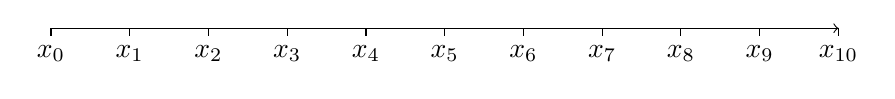
\begin{tikzpicture}
    \draw[->] (0,0) -- (10,0);
    \foreach \x in {0,1,2,3,4,5,6,7,8,9,10}
        \draw (\x,0) -- (\x,-0.1) node[below] {$x_{\x}$};


\end{tikzpicture}


$(x_i)_{i \in \llbracket 0, N + 1 \rrbracket}$, coordonnées des noeuds de maillage. \\

On cherche $u_h \in \mathbb{R}^{N+2}$, approximation de $u$ en $(x_i)_{i \in \llbracket 0, N + 1 \rrbracket}$. \\
Les conditions aux limites donnent : 
\boxed{
        u_0 = u_{N+1} = 0 \\
}\\

Il nous reste à trouver $(u_i)_{i \in \llbracket 1, N \rrbracket}$ avec $u_h = (u_i)_{i \in \llbracket 0, N + 1 \rrbracket}$. \\


On approxime $u''(x_i) \forall i \in \llbracket 1, N \rrbracket$ par : \\
$u''(x_i) \approx \frac{u(x_{i+1}) - 2u(x_i) + u(x_{i-1})}{h^2}$. (Hypothèse que $u \in \mathcal{C}^4(]0, 1[)$) \\


D'où  la résolution de $(P)$ revient à résoudre : \\

\begin{equation}
    (P_h) \qquad
    \begin{cases}
        -\frac{u_{i+1} - 2u_i + u_{i-1}}{h^2} + c(x_i)u_i = f(x_i) & \forall i \in \llbracket 1, N \rrbracket \\
        u_0 = u_{N+1} = 0
    \end{cases}
    \label{eq:Ph}
\end{equation}


\remarque{
    Etude de la consistence, stabilité (instationnaire) et convergence du schéma numérique.
}

\remarque{
    Limitations :
    \begin{itemize}
        \item $u$ supposé "suffisamment régulière" pour que l'approximation de $u''$ soit correcte. (Est-on contraint apr une telle hypothèse pour la résolution numérique ?)
        \item Grille régulière : problème d'adéquation entre la grille spatiale et la frontière du domaine.
    \end{itemize}
}

\subsection{ModIA 5 : Formulation variationnelle et méthode des éléments finis}

\subsubsection{Construction d'un "nouveau" problème}

\important{
    Trouver $u \in V$ tel que :
    \begin{equation}
        (P_{FV}) \qquad
        \forall v \in V, \quad -\int_{\Omega} u''(x)v(x)dx + \int_{\Omega} c(x)u(x)v(x)dx = \int_{\Omega} f(x)v(x)dx
        \label{eq:V}
    \end{equation}
}

\underline{Questions :}
\begin{itemize}
    \item Dans quel espace choisir $u$ et $v$ pour que les intégrales soient bien définies ?
    \item Condition d'existence et unicité de la solution de ce problème
    \item Lien entre la solution de $(P_{FV})$ et celle de $(P)$ ?
\end{itemize}


\subsubsection{Résolution numérique de $(P_{FV})$}
Recherche d'une solution à $(P_{FV})$ sur un sous-espace de dimension finie.

\underline{Questions :}
\begin{itemize}
    \item Comment construire ce sous-espace ?
    \item Convergence de la méthode ?
\end{itemize}


\section{Espace $L^2(\Omega)$ et dérivée faible}

\subsection{Espace des fonctions tests}

\definition{- Espace des fonctions tests}{
    On note $D(\Omega)$ l'espace des fonctions "tests", définiés sur $\Omega$, $\mathcal{C}^{\infty}$ et à support compact $K$ inclus dans $\Omega$. \\
    $D(\Omega)$ est un espace vectoriel.
}

\remarque{
    \begin{enumerate}[label=\roman*)]
        \item Support d'une fonction $\psi : \Omega \rightarrow \mathbb{R}$ : $\text{supp}(\psi) = \overline{\{x \in \Omega, \psi(x) \neq 0\}}$.
        \item Soit $\psi \in D(\Omega)$, alors toutes ses dérivées sont des fonctions tests.
    \end{enumerate}
}

\definition{- Convergence dans $D(\Omega)$}{
    Soient $\psi \in D(\Omega)$ et $(\psi_p) \in D(\Omega)^{\mathbb{N}}$. \\
    On dit que $(\psi_p)$ converge vers $\psi$ dans $D(\Omega)$ si :
    \begin{enumerate}[label=\roman*)]
        \item $\exists K \subset \Omega$ compact tel que $\forall p \in \mathbb{N}, \text{supp}(\psi_p) \subset K$ et $\text{supp}(\psi) \subset K$.
        \item $\forall \alpha \in \mathbb{N}^n$, $(D^\alpha \psi_p)$ converge uniformément vers $D^\alpha \psi$ sur $K$.\\
        
        $\Leftrightarrow \forall \alpha \in \mathbb{N}^n, \forall \varepsilon > 0, \exists p_0 \in \mathbb{N} \text{ tel que } \forall p \geq p_0$,\\
        $\forall x \in \Omega, |D^\alpha \psi_p(x) - D^\alpha \psi(x)| < \varepsilon$.\\
    \end{enumerate}

    avec $D^\alpha \psi = \frac{\partial^{|\alpha|}}{\partial x_1^{\alpha_1} \ldots \partial x_n^{\alpha_n}} \psi$.
}

\noindent\textbf{Exemple :} $n = 2$
\begin{itemize}
    \item $\alpha = (1, 0)$, $D^\alpha \psi = \frac{\partial \psi}{\partial x_1}$.
    \item $\alpha = (1, 1)$, $D^\alpha \psi = \frac{\partial^2 \psi}{\partial x_1 \partial x_2}$.
    \item $\alpha = (0, 2)$, $D^\alpha \psi = \frac{\partial^2 \psi}{\partial x_2^2}$.
\end{itemize}


\subsection{Espace $L^2(\Omega)$}

\definition{}{
    Soit $\Omega$ ouvert de $\mathbb{R}^n$ muni de la mesure de Lebesgue. \\
    On pose $\mathcal{L}^2(\Omega)$ l'ensemble des fonctions mesurables sur $\Omega$ : \\
    $\mathcal{L}^2(\Omega) = \{v : \Omega \rightarrow \mathbb{R} \text{ tel que } \int_{\Omega} |v(x)|^2 dx < +\infty\}$. \\

    On introduit la relation d'équivalence $\sim$ sur $\mathcal{L}^2(\Omega)$, définie par :
    $$
    \forall (f, g) \in (\mathcal{L}^2(\Omega))^2, f \sim g \Leftrightarrow f = g \text{ p.p. sur } \Omega
    $$

    On définit $L^2(\Omega) := \mathcal{L}^2(\Omega) / \sim$.
    $$
    \forall f \in L^2(\Omega), f = \{g \in \mathcal{L}^2(\Omega) \text{ tel que } g = f \text{ p.p. sur } \Omega\}
    $$
    On identifie $f \in L^2(\Omega)$ avec son représentant $f$ sur $\mathcal{L}^2(\Omega)$.
}

\remarque{
    \begin{itemize}
        \item $\int_{\Omega} |f(x)|^2 dx = 0$ avec $f \in \mathcal{L}^2(\Omega) \Leftrightarrow f = 0 \text{ p.p. sur } \Omega$.
        \item $\int_{\Omega} |f(x)|^2 dx = 0$ avec $f \in L^2(\Omega) \Leftrightarrow f = 0$ sur $L^2(\Omega)$.
    \end{itemize}
}


\theoreme{}{
    $L^2(\Omega)$ muni du produit scalaire $\langle \cdot, \cdot \rangle$ défini par : \\
    $$
    \forall (f, g) \in (L^2(\Omega))^2, \langle f, g \rangle_{L^2(\Omega)} = \int_{\Omega} f(x)g(x)dx
    $$
    est un espace de Hilbert. \\
    On notera $\|f\|_{L^2(\Omega)} = \sqrt{\int_{\Omega} |f(x)|^2 dx}$ la norme associée.
}

\propriete{- Fonctions "tests" et $L^2(\Omega)$}{
    \begin{enumerate}[label=\roman*)]
        \item $D(\Omega) \subset L^2(\Omega)$.
        \item Soit $(\psi_p) \in D(\Omega)^{\mathbb{N}}$ qui converge (au sens de la convergence dans $D(\Omega)$) vers $\psi \in D(\Omega)$. \\
        Alors $(\psi_p)$ converge vers $\psi \in L^2(\Omega)$.
        \item $D(\Omega)$ est dense dans $L^2(\Omega)$ : \\
        $\forall f \in L^2(\Omega), \exists (f_p) \in D(\Omega)^{\mathbb{N}} \text{ tel que } \underset{p \rightarrow \infty}{\lim} \| f_p - f \|_{L^2(\Omega)} = 0$.
        \item Soit $f \in L^2(\Omega)$ telle que $\forall \psi \in D(\Omega), \int_{\Omega} f(x)\psi(x)dx = 0$. \\
        Alors $f = 0$ sur $L^2(\Omega)$.
    \end{enumerate}
}

\remarque{
    On notera $\psi_p \xrightarrow[p \rightarrow \infty]{D(\Omega)} \psi \Rightarrow \psi_p \xrightarrow[p \rightarrow \infty]{L^2(\Omega)} \psi$.
}


\subsection{Dérivée faible et divergence faible dans $L^2(\Omega)$}

\definition{- Dérivée faible}{
    Soit $v \in L^2(\Omega)$. \\
    On dit que $v$ admet une \textit{dérivée faible} dans $L^2(\Omega)$ si :
    $$
    \forall i \in \llbracket 1, n \rrbracket, \exists w_i \in L^2(\Omega) \text{ tel que } \forall \psi \in D(\Omega), \int_{\Omega} v(x) \frac{\partial \psi}{\partial x_i} dx = - \int_{\Omega} w_i(x) \psi(x) dx
    $$
    $\forall i \in \llbracket 1, n \rrbracket$, $w_i$ ainsi défini est appelé la \textit{i-ème dérivée partielle première faible} de $v$. On la notera $w_i := \frac{\partial v}{\partial x_i}$.
}

\remarque{
    \begin{enumerate}[label=\roman*)]
        \item $\forall v \in L^2(\Omega), \frac{\partial v}{\partial x_i}$ est un abus de langage renvoyant à la i-ème dérivée partielle faible.
        \item Si $v \in L^2(\Omega)$ est dérivable et $\forall i \in \llbracket 1, n \rrbracket, \frac{\partial v}{\partial x_i} \in L^2(\Omega)$, alors les dérivées partielles faibles et classiques coïncident.
    \end{enumerate}
}

\propriete{}{
    Soit $v \in L^2(\Omega)$. \\
    $v$ admet une dérivée faible dans $L^2(\Omega)$ si
    $$
    \exists c > 0 \text{ tel que } \forall \psi \in D(\Omega), \forall i \in \llbracket 1, n \rrbracket, \left| \int_{\Omega} v(x) \frac{\partial \psi}{\partial x_i} dx \right| \leq c \| \psi \|_{L^2(\Omega)}
    $$
}

\definition{- Divergence faible}{
    Soit $\sigma : \Omega \rightarrow \mathbb{R}^n$ telle que $\forall i \in \llbracket 1, n \rrbracket, \sigma_i \in L^2(\Omega)$. \\
    On notera également $\sigma \in \left[L^2(\Omega)\right]^n$. \\
    On dit que $\sigma$ admet une \textit{divergence faible} dans $L^2(\Omega)$ si :
    $$
    \exists w \in L^2(\Omega) \text{ tel que } \forall \psi \in D(\Omega), \int_{\Omega} \sigma(x) \cdot \nabla \psi(x) dx = - \int_{\Omega} w(x) \psi(x) dx
    $$
    avec $\sigma \cdot \nabla \psi = \sum_{i=1}^n \sigma_i \frac{\partial \psi}{\partial x_i}$. \\

    $w \in L^2(\Omega)$ ainsi défini est appelé la \textit{divergence faible} de $\sigma$. On la notera $w := \text{div}(\sigma)$. ($\text{div}(v) = \sum_{i=1}^n \frac{\partial v}{\partial x_i}$)
}

\propriete{}{
    Soit $\sigma \in \left[L^2(\Omega)\right]^n$. \\
    $\sigma$ admet une divergence faible si
    $$
    \exists c > 0 \text{ tel que } \forall \psi \in D(\Omega), \left| \int_{\Omega} \sigma(x) \cdot \nabla \psi(x) dx \right| \leq c \| \psi \|_{L^2(\Omega)}
    $$
}


\section{Espaces de Sobolev}

\subsection{Espace $H^1(\Omega)$ et ses généralisations}

\definition{}{
    Soit $\Omega$ ouvert de $\mathbb{R}^n$. \\
    On appelle $H^1(\Omega)$ l'ensemble des éléments de $L^2(\Omega)$ qui admettent une dérivée faible dans $L^2(\Omega)$. \\
    On notera : $H^1(\Omega) = \{v \in L^2(\Omega) \text{ tel que } \forall i \in \llbracket 1, n \rrbracket, \frac{\partial v}{\partial x_i} \in L^2(\Omega)\}$.
}

\remarque{
    La notation $\frac{\partial v}{\partial x_i} \in L^2(\Omega)$ renvoie à l'existence d'une i-ème dérivée partielle faible de $v$.
}

\theoreme{}{
    $H^1(\Omega)$ muni du produit scalaire $\langle \cdot, \cdot \rangle$ défini par : \\
    $$
    \forall (f, g) \in (H^1(\Omega))^2, \langle f, g \rangle_{H^1(\Omega)} = \int_{\Omega} f(x)g(x)dx + \sum_{i=1}^n \int_{\Omega} \frac{\partial f}{\partial x_i}(x) \frac{\partial g}{\partial x_i}(x)dx
    $$
    est un espace de Hilbert.
}

\remarque{
    $\langle f, g \rangle_{H^1(\Omega)} = \langle f, g \rangle_{L^2(\Omega)} + \sum_{i=1}^n \langle \frac{\partial f}{\partial x_i}, \frac{\partial g}{\partial x_i} \rangle_{L^2(\Omega)}$. \\
}

\remarque{
    On note $\langle f, g \rangle_{1, \Omega} := \sum_{i=1}^n \langle \frac{\partial f}{\partial x_i}, \frac{\partial g}{\partial x_i} \rangle_{L^2(\Omega)}$. \\

    Cependant, $\langle f, g \rangle_{1, \Omega}$ n'est pas un produit scalaire sans autres hypothèses : $\langle f, f \rangle_{1, \Omega} = 0 \nRightarrow f = 0$.
}

\preuve{
    \begin{itemize}
        \item $H^1(\Omega)$ muni de $\langle \cdot, \cdot \rangle_{H^1(\Omega)}$ est un espace préhilbertien. (admis)
        \item $H^1(\Omega)$ muni de $\| \cdot \|_{H^1(\Omega)}$ défini par $\forall f \in H^1(\Omega), \| f \|_{H^1(\Omega)} = \sqrt{\| f \|_{L^2(\Omega)}^2 + \sum_{i=1}^n \| \frac{\partial f}{\partial x_i} \|_{L^2(\Omega)}^2}$ est complet : \\
        
        Soit $(u_p) \in H^1(\Omega)^{\mathbb{N}}$ une suite de Cauchy pour $\| \cdot \|_{H^1(\Omega)}$. \\
        Par définition, \\
        $\forall \varepsilon > 0, \exists p_0 \in \mathbb{N} \text{ tel que } \forall (p, q) \in \mathbb{N}^2, p, q \geq p_0 \Rightarrow \| u_p - u_q \|_{H^1(\Omega)} < \varepsilon$ \\

        Par définition de $\| \cdot \|_{H^1(\Omega)}$, \\
        $\forall \varepsilon > 0, \exists p_0 \in \mathbb{N} \text{ tel que } \forall (p, q) \in \mathbb{N}^2, p, q \geq p_0 \Rightarrow \| u_p - u_q \|_{L^2(\Omega)} < \varepsilon$ et $\| \frac{\partial u_p}{\partial x_i} - \frac{\partial u_q}{\partial x_i} \|_{L^2(\Omega)} < \varepsilon$ pour $i \in \llbracket 1, n \rrbracket$. \\

        Donc $(u_p)$ est une suite de Cauchy dans $L^2(\Omega)$ muni de $\| \cdot \|_{L^2(\Omega)}$ et ainsi converge dans $L^2(\Omega)$. On note $u \in L^2(\Omega)$ sa limite. \\

        De même, $\forall i \in \llbracket 1, n \rrbracket$, $(\frac{\partial u_p}{\partial x_i})$ est une suite de Cauchy dans $L^2(\Omega)$ et converge dans $L^2(\Omega)$. \\
        $\forall i \in \llbracket 1, n \rrbracket, \exists w_i \in L^2(\Omega) \text{ tel que } \frac{\partial u}{\partial x_i} \xrightarrow[p \rightarrow +\infty]{L^2(\Omega)} w_i$. \\

        Soit $p \in \mathbb{N}$. \\
        $\forall i \in \llbracket 1, n \rrbracket$, par définition de $\frac{\partial u_p}{\partial x_i}$, \\
        $\forall \psi \in D(\Omega), \int_{\Omega} u_p(x) \frac{\partial \psi}{\partial x_i} dx = - \int_{\Omega} \frac{\partial u_p}{\partial x_i}(x) \psi(x) dx$. \\

        D'où, $\int_{\Omega} \frac{\partial u_p}{\partial x_i}(x) \psi(x) dx = - \langle u_p, \frac{\partial \psi}{\partial x_i} \rangle_{L^2(\Omega)} \xrightarrow[p \rightarrow +\infty]{} - \langle u, \frac{\partial \psi}{\partial x_i} \rangle_{L^2(\Omega)}$. \\

        Or, $\langle u, \frac{\partial \psi}{\partial x_i} \rangle_{L^2(\Omega)} = \int_{\Omega} u(x) \frac{\partial \psi}{\partial x_i} dx$. \\
        De plus, $\int_{\Omega} \frac{\partial u_p}{\partial x_i}(x) \psi(x) dx = \langle \frac{\partial u_p}{\partial x_i}, \psi \rangle_{L^2(\Omega)} \xrightarrow[p \rightarrow +\infty]{} \langle w_i, \psi \rangle_{L^2(\Omega)}$. \\

        D'où, $\int_{\Omega} w_i \psi dx = - \int_{\Omega} u \frac{\partial \psi}{\partial x_i} dx$. \\
        $\Leftrightarrow \int_{\Omega} u \frac{\partial \psi}{\partial x_i} dx = - \int_{\Omega} w_i \psi dx$. \\

        \textit{Texte manquant}
    \end{itemize}
}

\remarque{
    \begin{enumerate}[label=\roman*)]
        \item Si $\Omega$ est borné, alors $\mathcal{C}^1(\overline{\Omega}) \subset H^1(\Omega)$.
        \item $H^1(\Omega) \subsetneq L^2(\Omega)$ (inclusion stricte).
        \item $D(\Omega)$ est un sous-espace vectoriel de $H^1(\Omega)$.\\
        $D(\Omega)$ n'est pas dense dans $H^1(\Omega)$.
    \end{enumerate}
}


\subsection{Espace $H^1_0(\Omega)$}

\definition{- Espace $H^1_0(\Omega)$}{
    $H^1_0(\Omega)$ est la fermeture de $D(\Omega)$ dans $H^1(\Omega)$. \\
    $$
    H^1_0(\Omega) = \overline{D(\Omega)}^{H^1(\Omega)} = \{v \in H^1(\Omega) \text{ tel que } \exists (v_p) \in D(\Omega)^{\mathbb{N}} \text{ tel que } v_p \xrightarrow[p \rightarrow +\infty]{H^1(\Omega)} v\}
    $$
}

\propriete{- Inégalité de Poincarré}{
    Soit $\Omega$ un ouvert borné de $\mathbb{R}^n$. \\
    $\exists C_{\Omega} > 0 \text{ tel que } \forall v \in H^1_0(\Omega), \| v \|_{L^2(\Omega)} \leq C_{\Omega} |v|_{1, \Omega}$. \\
    avec $|v|_{1, \Omega} = \sqrt{\sum_{i=1}^n \| \frac{\partial v}{\partial x_i} \|_{L^2(\Omega)}^2}$.
}

\preuve{
    admis (calcul intégral)
}

\remarque{
    Si $\Omega$ est un ouvert borné, $H^1_0(\Omega) \subsetneq H^1(\Omega)$ (exemple : fonction constante non-nulle). \\
    De plus, l'inégalité de Poincarré n'est pas valide pour $v \in H^1(\Omega) \backslash H^1_0(\Omega)$.
}

\important{
    \underline{Corollaire :}
    Soit $\Omega$ un ouvert borné de $\mathbb{R}^n$. \\
    La semi-norme $| \cdot |_{1, \Omega}$ est une norme sur $H^1_0(\Omega)$ équivalente à la norme induite par $\| \cdot \|_{H^1(\Omega)}$.
}

\theoreme{}{
    Soit $\Omega$ un ouvert borné de $\mathbb{R}^n$. \\
    $H^1_0(\Omega)$ muni du produit scalaire $\langle \cdot, \cdot \rangle_{1, \Omega}$ défini par :
    $$
    \forall (f, g) \in (H^1_0(\Omega))^2, \langle f, g \rangle_{1, \Omega} = \sum_{i=1}^n \int_{\Omega} \frac{\partial f}{\partial x_i}(x) \frac{\partial g}{\partial x_i}(x)dx
    $$
    est un espace de Hilbert.
}

\propriete{}{
    Soit $\Omega$ un ouvert borné de $\mathbb{R}^n$ à frontière Lipschitzienne. ($\Omega$ est appelé "domaine") \\
    Alors $D(\overline{\Omega})$ est dense dans $H^1(\Omega)$ pour la norme $\| \cdot \|_{H^1(\Omega)}$ \\
    avec $D(\overline{\Omega}) = \{\text{restriction des fonctions tests de } \mathbb{R}^n \text{ à } \Omega\}$.
}

\preuve{
    admis
}

\definition{}{
    Soit $m \in \mathbb{N}$. \\
    On appelle $H^m(\Omega) = \{v \in L^2(\Omega) \text{ tel que } \forall \alpha \in \mathbb{N}^n, | \alpha | \leq m, D^\alpha v \in L^2(\Omega)\}$.
}


\textit{Texte manquant}




\end{document}
